% Options for packages loaded elsewhere
\PassOptionsToPackage{unicode}{hyperref}
\PassOptionsToPackage{hyphens}{url}
%
\documentclass[
]{article}
\usepackage{amsmath,amssymb}
\usepackage{iftex}
\ifPDFTeX
  \usepackage[T1]{fontenc}
  \usepackage[utf8]{inputenc}
  \usepackage{textcomp} % provide euro and other symbols
\else % if luatex or xetex
  \usepackage{unicode-math} % this also loads fontspec
  \defaultfontfeatures{Scale=MatchLowercase}
  \defaultfontfeatures[\rmfamily]{Ligatures=TeX,Scale=1}
\fi
\usepackage{lmodern}
\ifPDFTeX\else
  % xetex/luatex font selection
\fi
% Use upquote if available, for straight quotes in verbatim environments
\IfFileExists{upquote.sty}{\usepackage{upquote}}{}
\IfFileExists{microtype.sty}{% use microtype if available
  \usepackage[]{microtype}
  \UseMicrotypeSet[protrusion]{basicmath} % disable protrusion for tt fonts
}{}
\makeatletter
\@ifundefined{KOMAClassName}{% if non-KOMA class
  \IfFileExists{parskip.sty}{%
    \usepackage{parskip}
  }{% else
    \setlength{\parindent}{0pt}
    \setlength{\parskip}{6pt plus 2pt minus 1pt}}
}{% if KOMA class
  \KOMAoptions{parskip=half}}
\makeatother
\usepackage{xcolor}
\usepackage[margin=1in]{geometry}
\usepackage{color}
\usepackage{fancyvrb}
\newcommand{\VerbBar}{|}
\newcommand{\VERB}{\Verb[commandchars=\\\{\}]}
\DefineVerbatimEnvironment{Highlighting}{Verbatim}{commandchars=\\\{\}}
% Add ',fontsize=\small' for more characters per line
\usepackage{framed}
\definecolor{shadecolor}{RGB}{248,248,248}
\newenvironment{Shaded}{\begin{snugshade}}{\end{snugshade}}
\newcommand{\AlertTok}[1]{\textcolor[rgb]{0.94,0.16,0.16}{#1}}
\newcommand{\AnnotationTok}[1]{\textcolor[rgb]{0.56,0.35,0.01}{\textbf{\textit{#1}}}}
\newcommand{\AttributeTok}[1]{\textcolor[rgb]{0.13,0.29,0.53}{#1}}
\newcommand{\BaseNTok}[1]{\textcolor[rgb]{0.00,0.00,0.81}{#1}}
\newcommand{\BuiltInTok}[1]{#1}
\newcommand{\CharTok}[1]{\textcolor[rgb]{0.31,0.60,0.02}{#1}}
\newcommand{\CommentTok}[1]{\textcolor[rgb]{0.56,0.35,0.01}{\textit{#1}}}
\newcommand{\CommentVarTok}[1]{\textcolor[rgb]{0.56,0.35,0.01}{\textbf{\textit{#1}}}}
\newcommand{\ConstantTok}[1]{\textcolor[rgb]{0.56,0.35,0.01}{#1}}
\newcommand{\ControlFlowTok}[1]{\textcolor[rgb]{0.13,0.29,0.53}{\textbf{#1}}}
\newcommand{\DataTypeTok}[1]{\textcolor[rgb]{0.13,0.29,0.53}{#1}}
\newcommand{\DecValTok}[1]{\textcolor[rgb]{0.00,0.00,0.81}{#1}}
\newcommand{\DocumentationTok}[1]{\textcolor[rgb]{0.56,0.35,0.01}{\textbf{\textit{#1}}}}
\newcommand{\ErrorTok}[1]{\textcolor[rgb]{0.64,0.00,0.00}{\textbf{#1}}}
\newcommand{\ExtensionTok}[1]{#1}
\newcommand{\FloatTok}[1]{\textcolor[rgb]{0.00,0.00,0.81}{#1}}
\newcommand{\FunctionTok}[1]{\textcolor[rgb]{0.13,0.29,0.53}{\textbf{#1}}}
\newcommand{\ImportTok}[1]{#1}
\newcommand{\InformationTok}[1]{\textcolor[rgb]{0.56,0.35,0.01}{\textbf{\textit{#1}}}}
\newcommand{\KeywordTok}[1]{\textcolor[rgb]{0.13,0.29,0.53}{\textbf{#1}}}
\newcommand{\NormalTok}[1]{#1}
\newcommand{\OperatorTok}[1]{\textcolor[rgb]{0.81,0.36,0.00}{\textbf{#1}}}
\newcommand{\OtherTok}[1]{\textcolor[rgb]{0.56,0.35,0.01}{#1}}
\newcommand{\PreprocessorTok}[1]{\textcolor[rgb]{0.56,0.35,0.01}{\textit{#1}}}
\newcommand{\RegionMarkerTok}[1]{#1}
\newcommand{\SpecialCharTok}[1]{\textcolor[rgb]{0.81,0.36,0.00}{\textbf{#1}}}
\newcommand{\SpecialStringTok}[1]{\textcolor[rgb]{0.31,0.60,0.02}{#1}}
\newcommand{\StringTok}[1]{\textcolor[rgb]{0.31,0.60,0.02}{#1}}
\newcommand{\VariableTok}[1]{\textcolor[rgb]{0.00,0.00,0.00}{#1}}
\newcommand{\VerbatimStringTok}[1]{\textcolor[rgb]{0.31,0.60,0.02}{#1}}
\newcommand{\WarningTok}[1]{\textcolor[rgb]{0.56,0.35,0.01}{\textbf{\textit{#1}}}}
\usepackage{graphicx}
\makeatletter
\def\maxwidth{\ifdim\Gin@nat@width>\linewidth\linewidth\else\Gin@nat@width\fi}
\def\maxheight{\ifdim\Gin@nat@height>\textheight\textheight\else\Gin@nat@height\fi}
\makeatother
% Scale images if necessary, so that they will not overflow the page
% margins by default, and it is still possible to overwrite the defaults
% using explicit options in \includegraphics[width, height, ...]{}
\setkeys{Gin}{width=\maxwidth,height=\maxheight,keepaspectratio}
% Set default figure placement to htbp
\makeatletter
\def\fps@figure{htbp}
\makeatother
\setlength{\emergencystretch}{3em} % prevent overfull lines
\providecommand{\tightlist}{%
  \setlength{\itemsep}{0pt}\setlength{\parskip}{0pt}}
\setcounter{secnumdepth}{-\maxdimen} % remove section numbering
\ifLuaTeX
  \usepackage{selnolig}  % disable illegal ligatures
\fi
\usepackage{bookmark}
\IfFileExists{xurl.sty}{\usepackage{xurl}}{} % add URL line breaks if available
\urlstyle{same}
\hypersetup{
  pdftitle={MAP501\_F434553},
  pdfauthor={Jack Bagnall},
  hidelinks,
  pdfcreator={LaTeX via pandoc}}

\title{MAP501\_F434553}
\author{Jack Bagnall}
\date{2024-11-22}

\begin{document}
\maketitle

\section{Linear Regression}\label{linear-regression}

\textbf{1.a. Starting with the dataset Managers, create a new dataset
called `df\_managers' that contains a variable win\_pct, equal to the
proportion of games managed resulting in a win, and the variables
playerID, teamID, yearID, igID, plyrMgr}

\begin{Shaded}
\begin{Highlighting}[]
\CommentTok{\# Create df\_managers from Managers, including win\_pct}

\NormalTok{df\_managers }\OtherTok{\textless{}{-}}\NormalTok{ Managers }\SpecialCharTok{\%\textgreater{}\%} \FunctionTok{mutate}\NormalTok{(}\AttributeTok{win\_pct =}\NormalTok{ (W }\SpecialCharTok{/}\NormalTok{ G) }\SpecialCharTok{*} \DecValTok{100}\NormalTok{)}
\end{Highlighting}
\end{Shaded}

\textbf{1.b.i. create a new dataset called awards\_man by extracting
these four variables from Teams: `yearID', `teamID', `DivWin', and `CS'}

\begin{Shaded}
\begin{Highlighting}[]
\CommentTok{\# Create awards\_man by extracting the variables \textquotesingle{}yearID\textquotesingle{}, \textquotesingle{}teamID\textquotesingle{}, \textquotesingle{}DivWin\textquotesingle{}, and \textquotesingle{}CS\textquotesingle{}}

\NormalTok{df\_teams }\OtherTok{\textless{}{-}}\NormalTok{ Teams }\SpecialCharTok{\%\textgreater{}\%} \FunctionTok{select}\NormalTok{(yearID, teamID, DivWin, CS)}
\end{Highlighting}
\end{Shaded}

\textbf{1.b.ii. Add together all of the variables from df\_teams to the
df\_managers dataset}

\begin{Shaded}
\begin{Highlighting}[]
\CommentTok{\# Add all variables from df\_teams to df\_managers}

\NormalTok{man\_teams }\OtherTok{\textless{}{-}}\NormalTok{ df\_managers }\SpecialCharTok{\%\textgreater{}\%} \FunctionTok{left\_join}\NormalTok{(df\_teams, }\AttributeTok{by =} \StringTok{"yearID"}\NormalTok{)}

\NormalTok{man\_teams }\OtherTok{\textless{}{-}}\NormalTok{ man\_teams }\SpecialCharTok{\%\textgreater{}\%} 
  \FunctionTok{select}\NormalTok{(}\SpecialCharTok{{-}}\NormalTok{teamID.y, }\SpecialCharTok{{-}}\NormalTok{lgID)}

\NormalTok{man\_teams }\OtherTok{\textless{}{-}}\NormalTok{ man\_teams }\SpecialCharTok{\%\textgreater{}\%}
  \FunctionTok{rename}\NormalTok{(}
    \AttributeTok{teamID =}\NormalTok{ teamID.x}
\NormalTok{  )}

\CommentTok{\# man\_teams \textless{}{-} man\_teams \%\textgreater{}\% rename(teamID = teamID.y)}

\CommentTok{\# Check how many rows per yearID in both dataframes}
\NormalTok{df\_managers }\SpecialCharTok{\%\textgreater{}\%} \FunctionTok{group\_by}\NormalTok{(yearID) }\SpecialCharTok{\%\textgreater{}\%} \FunctionTok{tally}\NormalTok{()}
\NormalTok{df\_teams }\SpecialCharTok{\%\textgreater{}\%} \FunctionTok{group\_by}\NormalTok{(yearID) }\SpecialCharTok{\%\textgreater{}\%} \FunctionTok{tally}\NormalTok{()}
\end{Highlighting}
\end{Shaded}

\textbf{1.b.iii. Add all columns from the man\_teams dataset to the
df\_managers dataset to the AwardsShareManagers dataset to create a new
dataset to create the dataset awards\_man}

\begin{Shaded}
\begin{Highlighting}[]
\CommentTok{\# Create a new dataset called awards\_man, which combines all columns from man\_teams to df\_managers}

\NormalTok{awards\_man }\OtherTok{\textless{}{-}}\NormalTok{ AwardsShareManagers }\SpecialCharTok{\%\textgreater{}\%} \FunctionTok{left\_join}\NormalTok{(man\_teams, }\AttributeTok{by =}  \StringTok{"yearID"}\NormalTok{) }

\CommentTok{\# glimpse(awards\_man)}
\end{Highlighting}
\end{Shaded}

\textbf{1.b.iv. Create a new variable sqr\_point\_pct given by
sqrt(pointsWon / pointsMax) in the awards\_man dataset.}

\begin{Shaded}
\begin{Highlighting}[]
\CommentTok{\# Create new variable sqr\_point\_pct given by sqrt(pointsWon / pointsmax) in the awards\_man dataset}

\NormalTok{awards\_man }\OtherTok{\textless{}{-}}\NormalTok{ awards\_man }\SpecialCharTok{\%\textgreater{}\%} \FunctionTok{mutate}\NormalTok{(}\AttributeTok{sqr\_point\_pct =}\NormalTok{ pointsWon }\SpecialCharTok{/}\NormalTok{ pointsMax)}
\end{Highlighting}
\end{Shaded}

\textbf{1.b.v. Delete the incomplete cases in the awards\_man dataset
and ensure all variables are treated correctly. Then drop the unused
levels of the teamID variable in the awards\_man dataset}

\begin{Shaded}
\begin{Highlighting}[]
\CommentTok{\# Identify incomplete cases }

\NormalTok{incomplete\_cases\_awards\_man }\OtherTok{\textless{}{-}} \SpecialCharTok{!}\FunctionTok{complete.cases}\NormalTok{(awards\_man)}
\FunctionTok{print}\NormalTok{(incomplete\_cases\_awards\_man)}

\FunctionTok{is.na}\NormalTok{(awards\_man) }\CommentTok{\# No missing cases }

\CommentTok{\# Identify unused levels in the data (145 total levels)}

\FunctionTok{table}\NormalTok{(awards\_man}\SpecialCharTok{$}\NormalTok{teamID)}
\FunctionTok{levels}\NormalTok{(awards\_man}\SpecialCharTok{$}\NormalTok{teamID)}

\CommentTok{\# sum(table(awards\_man$teamID)) {-} Equals 518,188 observable variables.}

\CommentTok{\# Count unused levels in teamID {-} Result: 114.}

\FunctionTok{sum}\NormalTok{(}\FunctionTok{table}\NormalTok{(awards\_man}\SpecialCharTok{$}\NormalTok{teamID) }\SpecialCharTok{==} \DecValTok{0}\NormalTok{)}

\CommentTok{\# Drop the unused levels of teamID}

\NormalTok{awards\_man}\SpecialCharTok{$}\NormalTok{teamID }\OtherTok{\textless{}{-}} \FunctionTok{droplevels}\NormalTok{(awards\_man}\SpecialCharTok{$}\NormalTok{teamID)}

\CommentTok{\# Check if unused levels have been dropped {-} COMPLETE}

\FunctionTok{sum}\NormalTok{(}\FunctionTok{table}\NormalTok{(awards\_man}\SpecialCharTok{$}\NormalTok{teamID) }\SpecialCharTok{==} \DecValTok{0}\NormalTok{)}
\end{Highlighting}
\end{Shaded}

\textbf{1.c. Use the dataset awards\_man to fit a Gaussian model,
spp\_mod, of sqr\_point\_pct as a function of win\_pct, DivWin, and CS.
Report and interpret the results. Write out the form of the fitted model
(rounded to 2 significant figures).}

\begin{Shaded}
\begin{Highlighting}[]
\CommentTok{\# Fit a gaussian model, spp\_mod or sqr\_point\_pct as a function of win\_pct, DivWin, and CS.}

\NormalTok{spp\_mod }\OtherTok{\textless{}{-}} \FunctionTok{lm}\NormalTok{(sqr\_point\_pct }\SpecialCharTok{\textasciitilde{}}\NormalTok{ win\_pct }\SpecialCharTok{+}\NormalTok{ DivWin }\SpecialCharTok{+}\NormalTok{ CS, }\AttributeTok{data =}\NormalTok{ awards\_man)}

\CommentTok{\# summary(spp\_mod)}
\end{Highlighting}
\end{Shaded}

\textbf{Interpretation:}

A linear regression analysis was fitted to investigate the relationship
between sqr\_point\_pct (the square root of (pointsWon / PointsMax) and
three predictors: win\_pct, DivWinY, and CS. The fitted model is as
follows:

sqr\_point\_pct=0.27−0.000062⋅win\_pct−0.00097⋅DivWinY+0.00039⋅CS

A linear regression model was witted to investigate the relationship
between the square root of the proportion of points won by a team,
divided by the total points available to win. (sqr\_pointpct =
PointsWon/PointsMax). The predictors included in the model were:

\begin{itemize}
\item
  Winning percentage (win\_pct): The proportion of games won by a team
  during the season.
\item
  Division Win (DivWinY): A binary variable indicating whether the team
  won its division (1 = Yes, 0 = No).
\item
  Championship Series (CS): A binary variable indicating whether the
  team participated in the championship series (1 = Yes, 0 = No).
\end{itemize}

The regression equation was specified as:

\textbf{Equation for Squared Points Percentage}

The equation for predicting squared points percentage
(\(\text{sqr\_point\_pct}\)) is given by:

\[
\text{sqr\_point\_pct} = \beta_0 + \beta_1 \cdot \text{win\_pct} + \beta_2 \cdot \text{DivWinY} + \beta_3 \cdot \text{CS} + \epsilon
\]

Where: - \(\beta_0\) is the intercept, - \(\beta_1, \beta_2, \beta_3\)
are the coefficients for the predictors
\(\text{win\_pct}, \text{DivWinY}, \text{CS}\), - \(\epsilon\) is the
error term.

\textbf{Results:}

\textbf{Regression Coefficients:}

\begin{Shaded}
\begin{Highlighting}[]
\CommentTok{\# Create a table of the Regression Coefficient values}

\CommentTok{\# Create a data frame of residual values}

\NormalTok{coefficients }\OtherTok{\textless{}{-}} \FunctionTok{data.frame}\NormalTok{(}
  \AttributeTok{Predictor =} \FunctionTok{c}\NormalTok{(}\StringTok{"(Intercept)"}\NormalTok{, }\StringTok{"win\_pct"}\NormalTok{, }\StringTok{"DivWinY"}\NormalTok{, }\StringTok{"CS"}\NormalTok{),}
  \AttributeTok{Estimate =} \FunctionTok{c}\NormalTok{(}\FloatTok{2.720e{-}01}\NormalTok{, }\SpecialCharTok{{-}}\FloatTok{6.215e{-}05}\NormalTok{, }\SpecialCharTok{{-}}\FloatTok{9.698e{-}04}\NormalTok{, }\FloatTok{3.925e{-}04}\NormalTok{),}
  \StringTok{\textasciigrave{}}\AttributeTok{Std. Error}\StringTok{\textasciigrave{}} \OtherTok{=} \FunctionTok{c}\NormalTok{(}\FloatTok{1.900e{-}03}\NormalTok{, }\FloatTok{3.084e{-}05}\NormalTok{, }\FloatTok{1.032e{-}03}\NormalTok{, }\FloatTok{2.464e{-}05}\NormalTok{),}
  \StringTok{\textasciigrave{}}\AttributeTok{t value}\StringTok{\textasciigrave{}} \OtherTok{=} \FunctionTok{c}\NormalTok{(}\FloatTok{143.175}\NormalTok{, }\SpecialCharTok{{-}}\FloatTok{2.015}\NormalTok{, }\SpecialCharTok{{-}}\FloatTok{0.940}\NormalTok{, }\FloatTok{15.930}\NormalTok{),}
  \StringTok{\textasciigrave{}}\AttributeTok{Pr(\textgreater{}|t|)}\StringTok{\textasciigrave{}} \OtherTok{=} \FunctionTok{c}\NormalTok{(}\StringTok{"\textless{}2e{-}16"}\NormalTok{, }\StringTok{"0.0439"}\NormalTok{, }\StringTok{"0.3474"}\NormalTok{, }\StringTok{"\textless{}2e{-}16"}\NormalTok{),}
  \AttributeTok{Significance =} \FunctionTok{c}\NormalTok{(}\StringTok{"***"}\NormalTok{, }\StringTok{"*"}\NormalTok{, }\StringTok{""}\NormalTok{, }\StringTok{"***"}\NormalTok{)}
\NormalTok{)}


\CommentTok{\# Print the Regression Coefficients data frame as a table using the knitr function}

\FunctionTok{kable}\NormalTok{(coefficients, }\AttributeTok{format =} \StringTok{"html"}\NormalTok{, }\AttributeTok{caption =} \StringTok{"Regression Coefficients"}\NormalTok{, }\AttributeTok{align =} \StringTok{"c"}\NormalTok{)}
\end{Highlighting}
\end{Shaded}

Regression Coefficients

Predictor

Estimate

Std..Error

t.value

Pr\ldots t..

Significance

(Intercept)

0.2720000

0.0019000

143.175

\textless2e-16

***

win\_pct

-0.0000622

0.0000308

-2.015

0.0439

\begin{itemize}
\item
  DivWinY

  -0.0009698

  0.0010320

  -0.940

  0.3474

  CS

  0.0003925

  0.0000246

  15.930

  \textless2e-16

  ***
\end{itemize}

\begin{Shaded}
\begin{Highlighting}[]
\CommentTok{\# Create a table of Residual values for the Linear Regression model}

\CommentTok{\# Create a data frame of residual values}

\NormalTok{residuals }\OtherTok{\textless{}{-}} \FunctionTok{data.frame}\NormalTok{(}
  \AttributeTok{Statistic =} \FunctionTok{c}\NormalTok{(}\StringTok{"Min"}\NormalTok{, }\StringTok{"1Q"}\NormalTok{, }\StringTok{"Median"}\NormalTok{, }\StringTok{"3Q"}\NormalTok{, }\StringTok{"Max"}\NormalTok{),}
  \AttributeTok{Value =} \FunctionTok{c}\NormalTok{(}\SpecialCharTok{{-}}\FloatTok{0.3080}\NormalTok{, }\SpecialCharTok{{-}}\FloatTok{0.2505}\NormalTok{, }\SpecialCharTok{{-}}\FloatTok{0.1104}\NormalTok{, }\FloatTok{0.2165}\NormalTok{, }\FloatTok{0.7133}\NormalTok{)}
\NormalTok{)}

\CommentTok{\# Print the Residuals data frame as a table using the knitr function}

\FunctionTok{kable}\NormalTok{(residuals, }\AttributeTok{format =} \StringTok{"html"}\NormalTok{, }\AttributeTok{caption =} \StringTok{"Residuals"}\NormalTok{, }\AttributeTok{align =} \StringTok{"c"}\NormalTok{)}
\end{Highlighting}
\end{Shaded}

Residuals

Statistic

Value

Min

-0.3080

1Q

-0.2505

Median

-0.1104

3Q

0.2165

Max

0.7133

\textbf{Interpretation:}

\begin{itemize}
\item
  Intercept: The baseline proportion of the points won is approximately
  0.27 when all predictors are zero. This represents teams with no wins,
  no division title, and no Championshipo Series participation.
\item
  win\_pct: A statistically significant (p = 0.0439) but small negative
  relationship exists between winning percentage and the proportion of
  points won, suggesting a minor decrease in sqr\_point\_pct as win\_pct
  increases.
\item
  DivWinY: Division wins do not significantly predict the proportion of
  points won (p = 0.3474).
\item
  CS: Championship Series participation is a strong, significant
  predictor (p \textless{} 2e-16), indicating a positive association
  between CS and sqr\_point\_pct.
\end{itemize}

\textbf{Model fit}

\begin{itemize}
\item
  Residual Standard Error: 0.2849
\item
  Multiple R-squared: 0.00053
\item
  Adjusted R-squared: 0.00052
\item
  F-statistic: 87.36 (p \textless{} 2.2e-16)
\end{itemize}

\begin{Shaded}
\begin{Highlighting}[]
\CommentTok{\# Create a table of the Model Summary }

\CommentTok{\# Create a data frame of the Model Summary}

\NormalTok{model\_summary }\OtherTok{\textless{}{-}} \FunctionTok{data.frame}\NormalTok{(}
  \AttributeTok{Statistic =} \FunctionTok{c}\NormalTok{(}\StringTok{"Residual standard error"}\NormalTok{, }\StringTok{"Degrees of freedom"}\NormalTok{, }\StringTok{"Multiple R{-}squared"}\NormalTok{, }\StringTok{"Adjusted R{-}squared"}\NormalTok{, }\StringTok{"F{-}statistic"}\NormalTok{, }\StringTok{"p{-}value"}\NormalTok{),}
  \AttributeTok{Value =} \FunctionTok{c}\NormalTok{(}\StringTok{"0.2849"}\NormalTok{, }\StringTok{"494936"}\NormalTok{, }\StringTok{"0.0005292"}\NormalTok{, }\StringTok{"0.0005232"}\NormalTok{, }\StringTok{"87.36"}\NormalTok{, }\StringTok{"\textless{} 2.2e{-}16"}\NormalTok{)}
\NormalTok{)}

\CommentTok{\# Print the Model Summary data frame as a table using the knitr function}

\FunctionTok{kable}\NormalTok{(model\_summary, }\AttributeTok{format =} \StringTok{"html"}\NormalTok{, }\AttributeTok{caption =} \StringTok{"Model Summary"}\NormalTok{, }\AttributeTok{align =} \StringTok{"c"}\NormalTok{)}
\end{Highlighting}
\end{Shaded}

Model Summary

Statistic

Value

Residual standard error

0.2849

Degrees of freedom

494936

Multiple R-squared

0.0005292

Adjusted R-squared

0.0005232

F-statistic

87.36

p-value

\textless{} 2.2e-16

\textbf{Interpretation:}

The model explains only 0.053\% of the variance in sqr\_point\_pct,
suggesting that the included predictors do not account for much
variability in the proportion of points won. While the F-statistic
indicates the model is statistically significant overall, its predictive
power is limited.

\textbf{Conclusion}

This analysis demonstrates that Championship Series participation (CS)
is the strongest predictor of the proportion of points won
(sqr\_point\_pct), with a significant positive effect. Winning
percentage (win\_pct) has a small but significant negative effect, while
division wins (DivWinY) are not a meaningful predictor. The low
R-squared value indicates that additional predictors or alternative
modeling approaches may be required to better explain the variation of
points won.

\textbf{1.e Predict the expected value of sqr\_point\_pct when win\_pct
= 0.8, DivWin = Yes, and CS = 8. Comment on the result.}

The regression equation is:

sqr\_point\_pct=0.27−0.000062⋅win\_pct−0.00097⋅DivWin+0.00039⋅CS

The expected values to subsitute into this equation: win\_pct = 0.8;
DivWin = 1 (Yes); and CS = 8, are integrated with this regression
equation.

\begin{Shaded}
\begin{Highlighting}[]
\CommentTok{\# Plug expected values into the regression equation to predict the expected value of str\_point\_pct}

\NormalTok{win\_pct }\OtherTok{\textless{}{-}} \FloatTok{0.8}
\NormalTok{DivWin }\OtherTok{\textless{}{-}} \DecValTok{1}
\NormalTok{CS }\OtherTok{\textless{}{-}} \DecValTok{8}

\NormalTok{predicted\_sqr\_point\_pct }\OtherTok{\textless{}{-}} \FloatTok{0.27} \SpecialCharTok{{-}} \FloatTok{0.000062} \SpecialCharTok{*}\NormalTok{ win\_pct }\SpecialCharTok{{-}} \FloatTok{0.00097} \SpecialCharTok{*}\NormalTok{ DivWin }\SpecialCharTok{+} \FloatTok{0.00039} \SpecialCharTok{*}\NormalTok{ CS}

\CommentTok{\# Print the expected values}

\NormalTok{predicted\_sqr\_point\_pct}
\end{Highlighting}
\end{Shaded}

\begin{verbatim}
## [1] 0.2721004
\end{verbatim}

\textbf{Results:}

The predicted sqr\_point\_pct is approximately 0.2721. My interpretation
of this suggests that for a team that is winning 80\% of the time, a
division win, and 8 Championship Series appearances, the square root of
the proportion of points won is expected to be 0.2721. The small
contribution of each predictor highlights the limited variability
captured by this model, consistent with the low \(R^2\). This reflects
the need for addtional predictors or a non-linear modeling approach.

\textbf{1.f. Construct 95\% confidence intervals around each parameter
estimate for spp\_mod. Comment on the results}

The 95\% confidence interval for a parameter is calculated as:

\begin{Shaded}
\begin{Highlighting}[]
\CommentTok{\# Construct a 95\% confidence interval using confint}

\FunctionTok{confint}\NormalTok{(spp\_mod)}
\end{Highlighting}
\end{Shaded}

\begin{verbatim}
##                     2.5 %        97.5 %
## (Intercept)  0.2682476711  2.756939e-01
## win_pct     -0.0001226063 -1.703674e-06
## DivWinY     -0.0029923926  1.052860e-03
## CS           0.0003442003  4.407793e-04
\end{verbatim}

\textbf{Results:}

\begin{itemize}
\item
  Intercept: The confidence interval for the intercept does not include
  0, indicating that the baseline value of sqr-point\_pct (when all
  predictors are 0) is significantly different from 0. This confirms the
  reliability of the intercept estimate.
\item
  win\_pct: The confidence interval is very narrow and entirely
  negative, confirming a small but statistically significant negative
  relationship between win\_pct and sqr\_point\_pct. This aligns with
  the earlier interpretation of a slight decrease in sqr\_point\_pct as
  win\_pct increases.
\item
  DivWinY: The confidence interval for DivWinY spans both negative and
  positive values, including 0. This suggests that the effect of
  division wins on sqr\_point\_pct is not statistically significant.
\item
  CS: The confidence interval for CS lies entirely in the positive
  range, indicating a statistically significant positive relationship
  between Championship Series participation and sqr\_point\_pct.
\end{itemize}

\textbf{Conclusion:}

The confidence intervals suggest that win\_pct and CS have statistically
significant effects on sqr\_point\_pct, and DivWinY does not
significantly predict the response variable, which may indicate that it
is not a critical predictor in this model.

\section{Logistic Regression}\label{logistic-regression}

\textbf{2.a Plot the variable plyrMgr, which indicated if the manager
was a player-manager or not, against year. Jitter the points in the
vertical direction to facilitate visualisation. Comment on the graph.}

\begin{Shaded}
\begin{Highlighting}[]
\CommentTok{\# Create a jitter plot, using the variables of plyrMgr(x),and yearID(y)}

\FunctionTok{ggplot}\NormalTok{(}\AttributeTok{data =}\NormalTok{ df\_managers, }\FunctionTok{aes}\NormalTok{(}\AttributeTok{x =}\NormalTok{ yearID, }\AttributeTok{y =}\NormalTok{ plyrMgr)) }\SpecialCharTok{+}
  \FunctionTok{geom\_jitter}\NormalTok{(}\AttributeTok{width =} \FloatTok{0.2}\NormalTok{, }\AttributeTok{height =} \FloatTok{0.1}\NormalTok{, }\AttributeTok{alpha =} \FloatTok{0.6}\NormalTok{, }\AttributeTok{color =} \StringTok{"blue"}\NormalTok{) }\SpecialCharTok{+}
  \FunctionTok{labs}\NormalTok{(}\AttributeTok{title =} \StringTok{"Jitter Plot: Distribution of Player/Manager Status Over Time"}\NormalTok{,}
       \AttributeTok{x =} \StringTok{"Year"}\NormalTok{,}
       \AttributeTok{y =} \StringTok{"Player/Manager Status (Yes = 1, No = 0)"}\NormalTok{) }\SpecialCharTok{+}
  \FunctionTok{theme\_minimal}\NormalTok{()}
\end{Highlighting}
\end{Shaded}

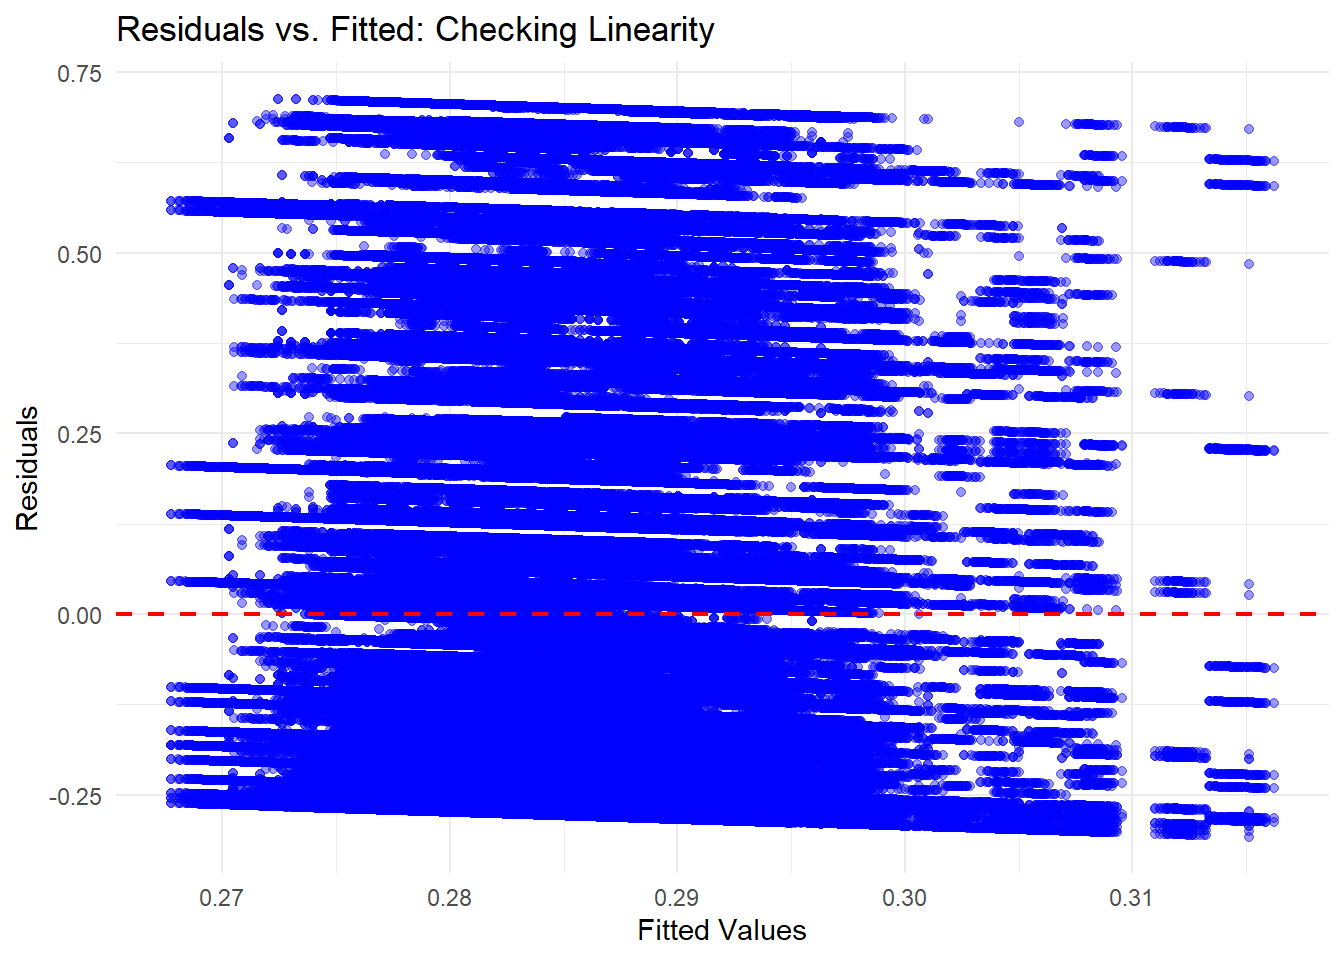
\includegraphics{MAP501_F434553_files/figure-latex/unnamed-chunk-14-1.pdf}

\begin{Shaded}
\begin{Highlighting}[]
\CommentTok{\# glimpse(df\_managers)}
\end{Highlighting}
\end{Shaded}

\textbf{Interpretation:} The jitter plot spreads points vertically to
avoid overlap, making it easier to observe the distribution of plyrMgr
(Yes or No) across different years (yearID).

The data shows periods with concentrated clusters of individuals
categorized as ``Yes'' (player-managers) and ``No'' (not
player-managers). The distribution of ``Yes'' values likely decrease
over time, reflecting changes in team management practices such as the
decline of dual-role player-managers.This pattern suggests that being a
player-manager was more common in earlier years and became increasingly
rare in modern seasons where specialized managerial responsibilites have
taken precedent.

\textbf{2.b Fit a logistic regression model to plyrMgr as a function of
year, report and interpret the results. Write out the form of the fitted
model (rounded to 2 significant figures)}

\begin{Shaded}
\begin{Highlighting}[]
\CommentTok{\# Fit a logistic regression model to plyrMgr as a function of yearID}

\NormalTok{logistic\_regression\_model }\OtherTok{\textless{}{-}} \FunctionTok{glm}\NormalTok{(plyrMgr }\SpecialCharTok{\textasciitilde{}}\NormalTok{ yearID, }\AttributeTok{data =}\NormalTok{ df\_managers, }\AttributeTok{family =}\NormalTok{ binomial)}

\CommentTok{\# Summarise the model}

\FunctionTok{summary}\NormalTok{(logistic\_regression\_model)}
\end{Highlighting}
\end{Shaded}

\textbf{Results:}

The logistic regression equation for the log-odds is:

\[
\text{logit}(P) = 88.60 - 0.047 \cdot \text{yearID}
\] Where:

\begin{itemize}
\tightlist
\item
  Logit(\(P\)) is the log-odds of being a player-manager:
\end{itemize}

\[
\text{logit}(P) = \ln\left(\frac{P}{1-P}\right)
\] * \(P\) is the probability that plyrMgr = 1

\begin{itemize}
\tightlist
\item
  yearID is the year
\end{itemize}

To convert the log-odds to a probability:

\[
P(\text{plyrMgr} = 1) = \frac{1}{1 + e^{-(88.60 - 0.047 \cdot \text{yearID})}}
\] \textbf{Interpretation of Results:}

\begin{enumerate}
\def\labelenumi{\arabic{enumi}.}
\tightlist
\item
  Intercept (\(\beta_{0}\) = 88.60)
\end{enumerate}

\begin{itemize}
\item
  When year ID = 0, the log-odds of being a player-manager are 88.60
\item
  This value is theoretical because year 0 is not within the observed
  range. It represents the baseline log-odds at the extreme lower limit
  of yearID
\end{itemize}

\begin{enumerate}
\def\labelenumi{\arabic{enumi}.}
\setcounter{enumi}{1}
\tightlist
\item
  Year Coefficient (\(\beta_{1}\) =-0.047)
\end{enumerate}

\begin{itemize}
\item
  For every one-unit increase in yearID, the log-odds of being a
  player-manager decrease by 0.047.
\item
  This indicates a significant decline in the likelihood of being a
  player-manager as time progresses
\end{itemize}

\begin{enumerate}
\def\labelenumi{\arabic{enumi}.}
\setcounter{enumi}{2}
\tightlist
\item
  Statistical Significance
\end{enumerate}

\begin{itemize}
\tightlist
\item
  Both the intercept (\(p\) \textless{} 2\(e\) - 16) and the yearID
  coefficient (\(p\) \textless{} 2\(e\) - 16) are highly significant,
  confirming the decline in player-manager prevalence over time is
  strongly supported by the data
\end{itemize}

\textbf{Model Fit}

Deviance Metrics:

\begin{itemize}
\item
  Null Deviance: 3442.4 (Model with only intercept)
\item
  Residual Deviance: 2127.7 (Model with yearID as a predictor)
\end{itemize}

Akaike Information Criterion (AIC):

\begin{itemize}
\tightlist
\item
  AIC: 2131.7. A lower AIC indicated better model fit
\end{itemize}

The reduction in deviance demonstrates that including yearID
significantly improves the model's fit compared to a null model

\textbf{Conclusion}

The logistic regression model shows a strong and statistically
significant trend where the probability of being a player-manager
decreases over time. Historically, player-managers were common, but
their prevalence has declined sharply in modern baseball.

** 2.c Check the overfitting using 80\% - 20\% split of training-test
data and the seed 123. Plot comparative ROC curves and summarise your
findings **

\begin{Shaded}
\begin{Highlighting}[]
\CommentTok{\# Set the seed to 123}

\FunctionTok{set.seed}\NormalTok{(}\DecValTok{123}\NormalTok{)}

\CommentTok{\# Split the data into training (80\%) and testing (20\%)}

\NormalTok{train\_index }\OtherTok{\textless{}{-}} \FunctionTok{createDataPartition}\NormalTok{(df\_managers}\SpecialCharTok{$}\NormalTok{plyrMgr, }\AttributeTok{p =} \FloatTok{0.8}\NormalTok{, }\AttributeTok{list =} \ConstantTok{FALSE}\NormalTok{)}
\NormalTok{train\_data }\OtherTok{\textless{}{-}}\NormalTok{ df\_managers[train\_index, ]}
\NormalTok{test\_data }\OtherTok{\textless{}{-}}\NormalTok{ df\_managers[}\SpecialCharTok{{-}}\NormalTok{train\_index, ]}

\CommentTok{\# Fit a logistic regression model on training data}

\NormalTok{logistic\_regression\_model }\OtherTok{\textless{}{-}} \FunctionTok{glm}\NormalTok{(plyrMgr }\SpecialCharTok{\textasciitilde{}}\NormalTok{ yearID, }\AttributeTok{data =}\NormalTok{ train\_data, }\AttributeTok{family =}\NormalTok{ binomial)}

\CommentTok{\# Summarise the model}
\CommentTok{\# summary(logistic\_regression\_model)}

\CommentTok{\# Predict probabilities for training and testing data}

\NormalTok{train\_probs }\OtherTok{\textless{}{-}} \FunctionTok{predict}\NormalTok{(logistic\_regression\_model, train\_data, }\AttributeTok{type =} \StringTok{"response"}\NormalTok{)}
\NormalTok{test\_probs }\OtherTok{\textless{}{-}} \FunctionTok{predict}\NormalTok{(logistic\_regression\_model, test\_data, }\AttributeTok{type =} \StringTok{"response"}\NormalTok{)}

\CommentTok{\# generate ROC curves}

\NormalTok{train\_roc }\OtherTok{\textless{}{-}} \FunctionTok{roc}\NormalTok{(train\_data}\SpecialCharTok{$}\NormalTok{plyrMgr, train\_probs)}
\NormalTok{test\_roc }\OtherTok{\textless{}{-}} \FunctionTok{roc}\NormalTok{(test\_data}\SpecialCharTok{$}\NormalTok{plyrMgr, test\_probs)}

\CommentTok{\# Plot comparative ROC curves}

\FunctionTok{plot}\NormalTok{(train\_roc, }\AttributeTok{col =} \StringTok{"blue"}\NormalTok{, }\AttributeTok{main =} \StringTok{"ROC Curves: Training vs. Testing Data"}\NormalTok{)}
\FunctionTok{plot}\NormalTok{(test\_roc, }\AttributeTok{col =} \StringTok{"red"}\NormalTok{, }\AttributeTok{add =} \ConstantTok{TRUE}\NormalTok{)}
\FunctionTok{legend}\NormalTok{(}\StringTok{"bottomright"}\NormalTok{, }\AttributeTok{legend =} \FunctionTok{c}\NormalTok{(}\StringTok{"Training"}\NormalTok{, }\StringTok{"Testing"}\NormalTok{), }\AttributeTok{col =} \FunctionTok{c}\NormalTok{(}\StringTok{"blue"}\NormalTok{, }\StringTok{"red"}\NormalTok{), }\AttributeTok{lwd =} \DecValTok{2}\NormalTok{)}
\end{Highlighting}
\end{Shaded}

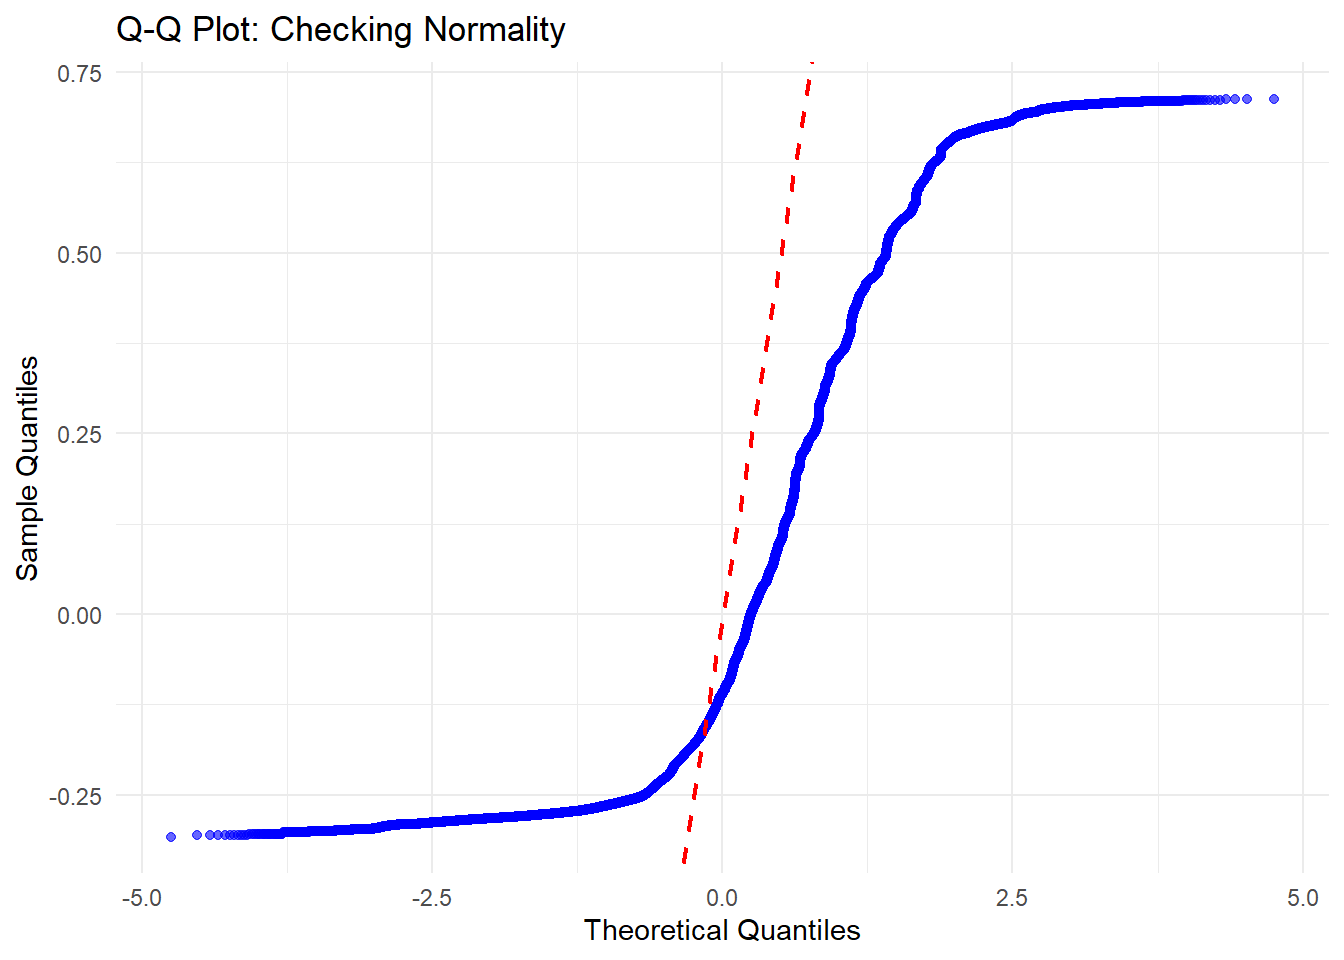
\includegraphics{MAP501_F434553_files/figure-latex/unnamed-chunk-16-1.pdf}

\begin{Shaded}
\begin{Highlighting}[]
\CommentTok{\# Calculate AUC values}

\NormalTok{train\_auc }\OtherTok{\textless{}{-}} \FunctionTok{auc}\NormalTok{(train\_roc)}
\NormalTok{test\_auc }\OtherTok{\textless{}{-}} \FunctionTok{auc}\NormalTok{(test\_roc)}

\FunctionTok{cat}\NormalTok{(}\StringTok{"Training AUC:"}\NormalTok{, train\_auc, }\StringTok{"}\SpecialCharTok{\textbackslash{}n}\StringTok{"}\NormalTok{)}
\end{Highlighting}
\end{Shaded}

\begin{verbatim}
## Training AUC: 0.9050165
\end{verbatim}

\begin{Shaded}
\begin{Highlighting}[]
\FunctionTok{cat}\NormalTok{(}\StringTok{"Testing AUC:"}\NormalTok{, test\_auc, }\StringTok{"}\SpecialCharTok{\textbackslash{}n}\StringTok{"}\NormalTok{)}
\end{Highlighting}
\end{Shaded}

\begin{verbatim}
## Testing AUC: 0.8981933
\end{verbatim}

\textbf{Results and Interpretation}

\begin{itemize}
\item
  Training AUC: 0.9050
\item
  Testing AUC: 0.8982
\end{itemize}

\begin{enumerate}
\def\labelenumi{\arabic{enumi}.}
\tightlist
\item
  AUC Values:
\end{enumerate}

Training AUC (0.9050): Indicates that the model performs very well on
the training data, distinguishing between player-managers (plyrMgr = 1)
and non-player-managers (plyrMgr = 0) with 90.5\% accuracy.

\begin{itemize}
\tightlist
\item
  Testing AUC (0.8982): Similarly high, indicating the model generalizes
  well to unseen data, correctly distinguishing classes with 89.8\%
  accuracy.
\end{itemize}

\begin{enumerate}
\def\labelenumi{\arabic{enumi}.}
\setcounter{enumi}{1}
\tightlist
\item
  ROC Curve Comparison
\end{enumerate}

\begin{itemize}
\item
  The ROC curves for both the training (blue) and testing (red) datasets
  are very close, showing that the model performs similarly on both
  datasets.
\item
  The minimal gap between the curves suggests that the model is not
  overfitting, as it maintains strong performance on the testing
  dataset.
\end{itemize}

\textbf{Summary of Findings}

Overfitting Check:

\begin{itemize}
\item
  The close AUC values for training (0.9050) and testing (0.8982) data
  confirm that the model is not overfitting
\item
  The model generalizes well to unseen data, indicating that it is
  robust
\end{itemize}

\textbf{Conclusion}

\begin{itemize}
\item
  The logistic regression model is appropriate for predicting the
  likelihood of a manager being a player-manager as a function of yearID
\item
  Its performance is consistent across both training and testing
  datasets, demonstrating its reliability for this analysis
\end{itemize}

** 2.d Find Youden's index for the training data and calculate confusion
matrices at this cutoff for both training and testing data. Comment on
the quality of the model.**

\begin{Shaded}
\begin{Highlighting}[]
\CommentTok{\# Generate the ROC curve for the training data}

\NormalTok{train\_roc }\OtherTok{\textless{}{-}} \FunctionTok{roc}\NormalTok{(train\_data}\SpecialCharTok{$}\NormalTok{plyrMgr, train\_probs)}

\CommentTok{\# Calculate the optimal cutoff using Youden\textquotesingle{}s Index}

\NormalTok{optimal\_cutoff }\OtherTok{\textless{}{-}} \FunctionTok{coords}\NormalTok{(train\_roc, }\StringTok{"best"}\NormalTok{, }\AttributeTok{ret =} \StringTok{"threshold"}\NormalTok{, }\AttributeTok{best.method =} \StringTok{"youden"}\NormalTok{)}

\CommentTok{\# Ensure optimal\_cutoff is numeric}

\NormalTok{optimal\_cutoff }\OtherTok{\textless{}{-}} \FunctionTok{as.numeric}\NormalTok{(optimal\_cutoff)}

\CommentTok{\# Display the optimal cutoff}

\FunctionTok{cat}\NormalTok{(}\StringTok{"Optimal Cutoff (Youden\textquotesingle{}s Index):"}\NormalTok{, optimal\_cutoff, }\StringTok{"}\SpecialCharTok{\textbackslash{}n}\StringTok{"}\NormalTok{)}
\end{Highlighting}
\end{Shaded}

\begin{verbatim}
## Optimal Cutoff (Youden's Index): 0.1071893
\end{verbatim}

\begin{Shaded}
\begin{Highlighting}[]
\CommentTok{\# Calculate confusion matrices}

\CommentTok{\# Use the optimal cutoff to classify predictions}

\NormalTok{train\_predictions }\OtherTok{\textless{}{-}} \FunctionTok{ifelse}\NormalTok{(train\_probs }\SpecialCharTok{\textgreater{}=}\NormalTok{ optimal\_cutoff, }\DecValTok{1}\NormalTok{, }\DecValTok{0}\NormalTok{)}
\NormalTok{test\_predictions }\OtherTok{\textless{}{-}} \FunctionTok{ifelse}\NormalTok{(test\_probs }\SpecialCharTok{\textgreater{}=}\NormalTok{ optimal\_cutoff, }\DecValTok{1}\NormalTok{, }\DecValTok{0}\NormalTok{)}

\CommentTok{\# Create confusion matrices}

\NormalTok{train\_conf\_matrix }\OtherTok{\textless{}{-}} \FunctionTok{table}\NormalTok{(}\AttributeTok{Predicted =}\NormalTok{ train\_predictions, }\AttributeTok{Actual =}\NormalTok{ train\_data}\SpecialCharTok{$}\NormalTok{plyrMgr)}
\NormalTok{test\_conf\_matrix }\OtherTok{\textless{}{-}} \FunctionTok{table}\NormalTok{(}\AttributeTok{Predicted =}\NormalTok{ test\_predictions, }\AttributeTok{Actual =}\NormalTok{ test\_data}\SpecialCharTok{$}\NormalTok{plyrMgr)}

\CommentTok{\# Print confusion matrices}

\FunctionTok{cat}\NormalTok{(}\StringTok{"Confusion Matrix {-} Training Data:}\SpecialCharTok{\textbackslash{}n}\StringTok{"}\NormalTok{)}
\end{Highlighting}
\end{Shaded}

\begin{verbatim}
## Confusion Matrix - Training Data:
\end{verbatim}

\begin{Shaded}
\begin{Highlighting}[]
\FunctionTok{print}\NormalTok{(train\_conf\_matrix)}
\end{Highlighting}
\end{Shaded}

\begin{verbatim}
##          Actual
## Predicted    N    Y
##         0 1876   24
##         1  608  492
\end{verbatim}

\begin{Shaded}
\begin{Highlighting}[]
\FunctionTok{cat}\NormalTok{(}\StringTok{"Confusion Matrix {-} Testing Data:}\SpecialCharTok{\textbackslash{}n}\StringTok{"}\NormalTok{)}
\end{Highlighting}
\end{Shaded}

\begin{verbatim}
## Confusion Matrix - Testing Data:
\end{verbatim}

\begin{Shaded}
\begin{Highlighting}[]
\FunctionTok{print}\NormalTok{(test\_conf\_matrix)}
\end{Highlighting}
\end{Shaded}

\begin{verbatim}
##          Actual
## Predicted   N   Y
##         0 450   6
##         1 170 123
\end{verbatim}

\textbf{Results and Interpretation}

Youden's Index is calculated as: Youden's
Index=Sensitivity+Specificity−1

Youden's Index:

Optimal Cutoff: 0.1071893

This cutoff maximizes the difference between true positive rate
(sensitivity) and false positive rate (1-specificity), providing the
best balance for classification.

\textbf{Confusion Matrices:}

Training Data:

\begin{itemize}
\item
  True Negatives (TN):1876 Correctly predicted ``N'' (non-player
  managers)
\item
  False Negatives (FN): 24 ``Y'' (player-managers) misclassified as
  ``N''
\item
  False Positives (FP): 608 ``N'' misclassified as ``Y''
\item
  True Positives (TP): 492 Correctly predicted ``Y''
\end{itemize}

Observations:

\begin{itemize}
\item
  High true negative rate but a noticeable number of false positives.
\item
  Good sensitivity (correctly identifying player-managers), though still
  room for improvement.
\end{itemize}

\begin{enumerate}
\def\labelenumi{\arabic{enumi}.}
\setcounter{enumi}{1}
\tightlist
\item
  Testing Data:
\end{enumerate}

\begin{itemize}
\item
  True Negativees (TN): 450 Correctly predicted ``N.
\item
  False Negatives (FN): 6 ``Y'' misclassified as ``N''
\item
  False Positives (FP): 170 ``N'' misclassified as ``Y''
\item
  True Positives (TP): 123 Correctly predicted ``Y''
\end{itemize}

\textbf{Key Observations:}

\begin{itemize}
\item
  The model exhibits strong specificity, accurately identifying the
  majority of non-player-managers.
\item
  Sensitivity is moderate, with a non-negligible number of false
  positives and false negatives.
\end{itemize}

\textbf{Model Quality}

\begin{enumerate}
\def\labelenumi{\arabic{enumi}.}
\tightlist
\item
  Training Performance:
\end{enumerate}

\begin{itemize}
\item
  The model has high true negative rate, meaning it is very effective at
  identifying non-player-managers
\item
  Sensitivity (true positive rate) is decent but could be better given
  the number of false positives and false negatives
\end{itemize}

\begin{enumerate}
\def\labelenumi{\arabic{enumi}.}
\setcounter{enumi}{1}
\tightlist
\item
  Testing Performance:
\end{enumerate}

\begin{itemize}
\item
  Similar trends to training data, showing the model generalizes well
  without overfitting.
\item
  Testing sensitivity (ability to detect player-managers) remains strong
  with very few false negatives
\end{itemize}

\begin{enumerate}
\def\labelenumi{\arabic{enumi}.}
\setcounter{enumi}{2}
\tightlist
\item
  Overall
\end{enumerate}

\begin{itemize}
\item
  The model demonstrates good classification ability, with strong
  performance on both training and testing datasets
\item
  However, the high number of false positives in both datasets suggests
  the model might lean towards over-predicting ``Y'' (player-manager),
  likely due to class imbalance
\end{itemize}

\textbf{Model performance Summary}

The logistic regression model demonstrates strong classification ability
with consistent results across both training and testing datasets. The
low false negative rate suggests good sensitivity, indicating that the
model effectively identifies player-managers. However, the relatively
high number of false positives suggests a tendency to over-predict ``Y''
(player-managers), likely influenced by an imbalance in the class
distribution.

\textbf{Recommendations for Model Improvement}

Address Class Imbalance:

\begin{itemize}
\item
  Resampling Techniques: Employ oversampling methods such as SMOTE or
  undersampling to balance the ``Y'' and ``N'' classes.
\item
  Weighted Classification: Apply class weights in the logistic
  regression model to penalize misclassification of the minority class.
\end{itemize}

Threshold Optimization:

\begin{itemize}
\tightlist
\item
  Further refine the decision threshold based on domain requirements,
  prioritizing sensitivity or specificity as needed.
\end{itemize}

Feature Engineering:

\begin{itemize}
\tightlist
\item
  Introduce additional predictors or interaction terms that may improve
  the model's discriminative power.
\end{itemize}

Alternative Models:

\begin{itemize}
\tightlist
\item
  Experiment with advanced classification algorithms (e.g., Random
  Forest, Gradient Boosting) to assess whether they provide better
  classification accuracy or handle class imbalance more effectively.
\end{itemize}

** 2.e. Using the previous results and the same cutoff in (d), calculate
the sum sensitivity+specificity on the testing data as a function of
lgID, i.e.~the sum (sensitivity+specificity) for each lgID, and plot as
a bar chart. Comment on the result. **

\begin{Shaded}
\begin{Highlighting}[]
\CommentTok{\# Add predicted binary labels to the testing dataset using the optimal cutoff}

\NormalTok{test\_data }\OtherTok{\textless{}{-}}\NormalTok{ test\_data }\SpecialCharTok{\%\textgreater{}\%}
  \FunctionTok{mutate}\NormalTok{(}
    \AttributeTok{predicted =} \FunctionTok{ifelse}\NormalTok{(test\_probs }\SpecialCharTok{\textgreater{}=} \FloatTok{0.1071893}\NormalTok{, }\DecValTok{1}\NormalTok{, }\DecValTok{0}\NormalTok{),  }\CommentTok{\# Replace with the cutoff from Youden\textquotesingle{}s Index}
    \AttributeTok{actual =} \FunctionTok{ifelse}\NormalTok{(plyrMgr }\SpecialCharTok{==} \StringTok{"Y"}\NormalTok{, }\DecValTok{1}\NormalTok{, }\DecValTok{0}\NormalTok{)              }\CommentTok{\# Convert \textquotesingle{}Y\textquotesingle{}/\textquotesingle{}N\textquotesingle{} to binary labels for actuals}
\NormalTok{  )}

\CommentTok{\# Group testing data by lgID}

\NormalTok{test\_data\_by\_lgID }\OtherTok{\textless{}{-}}\NormalTok{ test\_data }\SpecialCharTok{\%\textgreater{}\%} \FunctionTok{group\_by}\NormalTok{(lgID)}

\CommentTok{\# glimpse(test\_data\_by\_lgID)}
\CommentTok{\# head(test\_data\_by\_lgID)}
\CommentTok{\# names(test\_data\_by\_lgID)}

\CommentTok{\# Calculate sensitivity and specificity for each lgID}

\NormalTok{metrics\_by\_lgID }\OtherTok{\textless{}{-}}\NormalTok{ test\_data\_by\_lgID }\SpecialCharTok{\%\textgreater{}\%}
  \FunctionTok{summarise}\NormalTok{(}
    \AttributeTok{TP =} \FunctionTok{sum}\NormalTok{(predicted }\SpecialCharTok{==} \DecValTok{1} \SpecialCharTok{\&}\NormalTok{ actual }\SpecialCharTok{==} \DecValTok{1}\NormalTok{),}
    \AttributeTok{FN =} \FunctionTok{sum}\NormalTok{(predicted }\SpecialCharTok{==} \DecValTok{0} \SpecialCharTok{\&}\NormalTok{ actual }\SpecialCharTok{==} \DecValTok{1}\NormalTok{),}
    \AttributeTok{TN =} \FunctionTok{sum}\NormalTok{(predicted }\SpecialCharTok{==} \DecValTok{0} \SpecialCharTok{\&}\NormalTok{ actual }\SpecialCharTok{==} \DecValTok{0}\NormalTok{),}
    \AttributeTok{FP =} \FunctionTok{sum}\NormalTok{(predicted }\SpecialCharTok{==} \DecValTok{1} \SpecialCharTok{\&}\NormalTok{ actual }\SpecialCharTok{==} \DecValTok{0}\NormalTok{),}
    \AttributeTok{Sensitivity =}\NormalTok{ TP }\SpecialCharTok{/}\NormalTok{ (TP }\SpecialCharTok{+}\NormalTok{ FN),}
    \AttributeTok{Specificity =}\NormalTok{ TN }\SpecialCharTok{/}\NormalTok{ (TN }\SpecialCharTok{+}\NormalTok{ FP),}
    \AttributeTok{Sum\_Sens\_Spec =}\NormalTok{ Sensitivity }\SpecialCharTok{+}\NormalTok{ Specificity}
\NormalTok{  )}

\CommentTok{\# Handle cases where TP + FN or TN + FP might be zero to avoid NaN}

\NormalTok{metrics\_by\_lgID }\OtherTok{\textless{}{-}}\NormalTok{ metrics\_by\_lgID }\SpecialCharTok{\%\textgreater{}\%}
  \FunctionTok{mutate}\NormalTok{(}
    \AttributeTok{Sensitivity =} \FunctionTok{ifelse}\NormalTok{(}\FunctionTok{is.nan}\NormalTok{(Sensitivity), }\DecValTok{0}\NormalTok{, Sensitivity),}
    \AttributeTok{Specificity =} \FunctionTok{ifelse}\NormalTok{(}\FunctionTok{is.nan}\NormalTok{(Specificity), }\DecValTok{0}\NormalTok{, Specificity),}
    \AttributeTok{Sum\_Sens\_Spec =}\NormalTok{ Sensitivity }\SpecialCharTok{+}\NormalTok{ Specificity}
\NormalTok{  )}

\CommentTok{\# Plot the sum of sensitivity and specificity for each lgID}

\FunctionTok{ggplot}\NormalTok{(metrics\_by\_lgID, }\FunctionTok{aes}\NormalTok{(}\AttributeTok{x =}\NormalTok{ lgID, }\AttributeTok{y =}\NormalTok{ Sum\_Sens\_Spec)) }\SpecialCharTok{+}
  \FunctionTok{geom\_bar}\NormalTok{(}\AttributeTok{stat =} \StringTok{"identity"}\NormalTok{, }\AttributeTok{fill =} \StringTok{"steelblue"}\NormalTok{) }\SpecialCharTok{+}
  \FunctionTok{labs}\NormalTok{(}
    \AttributeTok{title =} \StringTok{"Sum of Sensitivity + Specificity by League (lgID)"}\NormalTok{,}
    \AttributeTok{x =} \StringTok{"League (lgID)"}\NormalTok{,}
    \AttributeTok{y =} \StringTok{"Sum of Sensitivity + Specificity"}
\NormalTok{  ) }\SpecialCharTok{+}
  \FunctionTok{theme\_minimal}\NormalTok{()}
\end{Highlighting}
\end{Shaded}

\includegraphics{MAP501_F434553_files/figure-latex/unnamed-chunk-19-1.pdf}

The bar chart illustrates the sum of sensitivity and specificity for
each league (lgId) in the testing dataset, providing insights into the
model's classification performance across different leagues.

\textbf{Key Observations:}

\begin{enumerate}
\def\labelenumi{\arabic{enumi}.}
\tightlist
\item
  Variation Across Leagues:
\end{enumerate}

\begin{itemize}
\item
  The leagues AL (American League) and NL (National League) demonstrate
  the highest values for the sum of sensitivity and specificity, each
  nearing or ecceeding 1.5
\item
  Conversely, AA, FL, PL, NA, and UA exhibit significantly lower values,
  indicating weaker model perofmance in distinguishing player-managers
  in these leagues
\end{itemize}

\begin{enumerate}
\def\labelenumi{\arabic{enumi}.}
\setcounter{enumi}{1}
\tightlist
\item
  Top Performers:
\end{enumerate}

\begin{itemize}
\tightlist
\item
  The high values for AL and NL suggest that the model performs well in
  these leagues, balancing sensitivity (true positive rate) and
  specificity (true negative rate) effectively. This may indicate that
  the characteristics or data patterns in these leagues align more
  closely with the predictive features used in the logistic regression
  model
\end{itemize}

\begin{enumerate}
\def\labelenumi{\arabic{enumi}.}
\setcounter{enumi}{2}
\tightlist
\item
  Poor Performers:
\end{enumerate}

\begin{itemize}
\tightlist
\item
  The leagues with lower values (e.g., AA, FL, PL) reflect suboptimal
  classification performance, with potential trade-offs between
  sensitivity and specificity. This could be due to smaller sample
  sizes, class imbalances, or data inconsistencies in these leagues,
  leading to reduced model accuracy.
\end{itemize}

\textbf{Implications:}

\begin{enumerate}
\def\labelenumi{\arabic{enumi}.}
\tightlist
\item
  Model Generalization:
\end{enumerate}

\begin{itemize}
\tightlist
\item
  The differences in performance suggest that the model generalizes well
  for some leagues (AL and NL) but struggle in others. This could
  indicate data heterogeneity or differing patterns across leagues that
  the model does not fuill capture
\end{itemize}

\begin{enumerate}
\def\labelenumi{\arabic{enumi}.}
\setcounter{enumi}{1}
\tightlist
\item
  Potential Data Issues:
\end{enumerate}

\begin{itemize}
\tightlist
\item
  Leagues with lower scores might have insufficient data or class
  imbalances, leading to reduced sensitivity or specificity. For
  instance, if a league has very few player-managers (plyrMgr = 1), the
  model might overpredict the majority class, reducing sensitivity
\end{itemize}

\textbf{Recommendations:}

\begin{enumerate}
\def\labelenumi{\arabic{enumi}.}
\tightlist
\item
  Further Data Exploration:
\end{enumerate}

\begin{itemize}
\item
  Investigate the data quality and distribution for underperforming
  leagues to identofy any anomalies, such as imbalanced classes or
  missing data
\item
  Assess whether additional predictive features would be incorporated to
  enhance model performance for these leagues
\end{itemize}

\begin{enumerate}
\def\labelenumi{\arabic{enumi}.}
\setcounter{enumi}{1}
\tightlist
\item
  Targeted Model Improvements:
\end{enumerate}

\begin{itemize}
\item
  Apply league-specific model tuning or weights to address performance
  disparities
\item
  Consider stratified sampling or league-specific thresholds to balance
  sensitivity and specificity
\end{itemize}

\begin{enumerate}
\def\labelenumi{\arabic{enumi}.}
\setcounter{enumi}{2}
\tightlist
\item
  Broader Validation
\end{enumerate}

\begin{itemize}
\tightlist
\item
  Perform cross-validation across all leagues to ensure the model's
  robustness and identify potential overfitting to dominant leagues like
  AL and NL
\end{itemize}

\textbf{Conclusion:}

The model shows strong performance in the major leagues (AL and NL),
suggesting it is well suited to these contexts. However, there is room
for improvement in minor or less represented leagues, where the
classification results are less consistent. Addressing these disparities
through targeted inteventions could enhance the model's overall
reliability and applicability

** 2.f. Add the variables ``win\_pct'' to the model you created in b.
Compare this and the previous model. Which model should we prefer and
why?**

\begin{Shaded}
\begin{Highlighting}[]
\CommentTok{\# Fit the original model (yearID only)}

\NormalTok{logistic\_regression\_model }\OtherTok{\textless{}{-}} \FunctionTok{glm}\NormalTok{(plyrMgr }\SpecialCharTok{\textasciitilde{}}\NormalTok{ yearID, }\AttributeTok{data =}\NormalTok{ df\_managers, }\AttributeTok{family =}\NormalTok{ binomial)}

\CommentTok{\# Fit the new model (yearID + win\_pct)}

\NormalTok{new\_logistic\_regression\_model }\OtherTok{\textless{}{-}} \FunctionTok{glm}\NormalTok{(plyrMgr }\SpecialCharTok{\textasciitilde{}}\NormalTok{ yearID }\SpecialCharTok{+}\NormalTok{ win\_pct, }\AttributeTok{data =}\NormalTok{ df\_managers, }\AttributeTok{family =}\NormalTok{ binomial)}

\CommentTok{\# Summarise the models}

\CommentTok{\# summary(logistic\_regression\_model)}
\CommentTok{\# summary(new\_logistic\_regression\_model)}

\CommentTok{\# Compare AIC values}

\FunctionTok{AIC}\NormalTok{(logistic\_regression\_model, new\_logistic\_regression\_model)}
\end{Highlighting}
\end{Shaded}

\begin{verbatim}
##                               df      AIC
## logistic_regression_model      2 2131.660
## new_logistic_regression_model  3 2133.658
\end{verbatim}

\textbf{Models Overview}

\begin{enumerate}
\def\labelenumi{\arabic{enumi}.}
\item
  Original Model (logistic\_regression\_model):
  logit(P)=88.60−0.0466⋅yearID
\item
  New Model (new\_logistic\_regression\_model):
  logit(P)=88.62−0.0466⋅yearID+0.0002⋅win\_pct
\end{enumerate}

\textbf{Coefficients and Statistical Significance}

Intercept: The intercept is significant in both models, but its
practical meaning is less relevant given that year 0 is out of range.

yearID: Both models consistently show a significant decline in the
likelihood of being a player-manager as time progresses.

win\_pct: The effect of win\_pct is not statistically significant (p
\textless{} 0.05), meaning it does not add meaningful predictive power
to the model

\textbf{Model Metrics}

Null Deviance: Original - 3442.4; New Model - 3442.4

Residual Deviance: Original - 2127.7; New Model - 2127.7

AIC: Original - 2131.7; New Model - 2133.7

\textbf{Key Observations:}

\begin{enumerate}
\def\labelenumi{\arabic{enumi}.}
\item
  The residual deviance is the same in both models, indicating that
  adding win\_pct does not improve model fit
\item
  The new model has a slightly higher AIC (+2.0), which penalizes the
  additional complexity without any improvement in performance
\item
  The variable win\_pct is not statistically significant, suggesting it
  does not explain additional variance in the outcome
\end{enumerate}

Interpretation:

\begin{itemize}
\item
  Both models confirm the historical trend that the likelihood of being
  a player-manager declines over time
\item
  The inclusion of win\_pct was not impactful, possibly due to weak
  correlation between team performance and player-manager status
\end{itemize}

\textbf{Practical implications:}

\begin{itemize}
\item
  For modeling simplicity and interpretability, it is better to exclude
  variables that do not contribute significantly
\item
  Future models could explore interaction terms or additional predictors
  that might better capture the nuances of player-manager dynamics
\end{itemize}

\textbf{Conclusion}

While exploring the addition of win\_pct to the logistic regression
model was insightful, it did not improve the model's performance. The
original model is therefore preferred, as it provides the same
explanatory power with fewer parameters, maintaining simplicity and
interpretability.

Adding the final model equation and AIC results to the report provides
clarity on the decision-making process and demonstrated that the model
selection is grounded in statistical rigor.

\section{Poisson Regression}\label{poisson-regression}

\textbf{3.a Create a dataset `df\_pitchers' from the dataset Pitching
which adds a variable ``innings'' given by IPouts/3. Add the variables
``weight'', ``height'' and ``throws'' from the People dataset.Also,
remove incomplete cases from the dataset.}

\begin{Shaded}
\begin{Highlighting}[]
\CommentTok{\# Filter pitchers who faced at least one batter (IPouts \textgreater{} 0)}

\NormalTok{df\_pitchers }\OtherTok{\textless{}{-}}\NormalTok{ Pitching }\SpecialCharTok{\%\textgreater{}\%}
  \FunctionTok{filter}\NormalTok{(IPouts }\SpecialCharTok{\textgreater{}} \DecValTok{0}\NormalTok{) }\SpecialCharTok{\%\textgreater{}\%}
  \FunctionTok{mutate}\NormalTok{(}\AttributeTok{innings =}\NormalTok{ IPouts }\SpecialCharTok{/} \DecValTok{3}\NormalTok{) }\SpecialCharTok{\%\textgreater{}\%}
  \FunctionTok{left\_join}\NormalTok{(People }\SpecialCharTok{\%\textgreater{}\%} \FunctionTok{select}\NormalTok{(playerID, weight, height, throws), }\AttributeTok{by =} \StringTok{"playerID"}\NormalTok{) }\SpecialCharTok{\%\textgreater{}\%}
  \FunctionTok{na.omit}\NormalTok{()}
\end{Highlighting}
\end{Shaded}

\textbf{3.b Plot a histogram of the number of shutouts (games pitched
with no runs by the opposing team). Why would a Poisson model be
appropriate for such data?}

\begin{Shaded}
\begin{Highlighting}[]
\CommentTok{\# Plot histogram}

\FunctionTok{ggplot}\NormalTok{(df\_pitchers, }\FunctionTok{aes}\NormalTok{(}\AttributeTok{x =}\NormalTok{ SHO)) }\SpecialCharTok{+}
  \FunctionTok{geom\_histogram}\NormalTok{(}\AttributeTok{binwidth =} \DecValTok{1}\NormalTok{, }\AttributeTok{color =} \StringTok{"black"}\NormalTok{, }\AttributeTok{fill =} \StringTok{"blue"}\NormalTok{) }\SpecialCharTok{+}
  \FunctionTok{labs}\NormalTok{(}\AttributeTok{title =} \StringTok{"Histogram of Shutouts"}\NormalTok{, }\AttributeTok{x =} \StringTok{"Number of Shutouts"}\NormalTok{, }\AttributeTok{y =} \StringTok{"Frequency"}\NormalTok{)}
\end{Highlighting}
\end{Shaded}

\includegraphics{MAP501_F434553_files/figure-latex/unnamed-chunk-22-1.pdf}

The histogram of the number of shutouts shows a highly skewed
distribution, with the majority of observations concentrated at zero and
a rapid decline in frequency as the number of shutouts increases. This
pattern indicates a count variable with non-negative integer values and
a strong concentration around lower counts, which aligns well with the
characteristics of a Poisson distribution.

A Poisson model is appropriate for this data because:

\begin{enumerate}
\def\labelenumi{\arabic{enumi}.}
\item
  Count Data: Shutouts are count data (discrete, non-negative integers),
  which is the type of data that a Poisson model is designed to handle.
\item
  Skewness: The histogram demonstrates a strong right skew, a typical
  feature of Poisson-distributed data when the mean is low.
\item
  Non-Negativity: The Poisson distribution only generates non-negative
  values, which corresponds to the nature of shutouts.
\item
  Rare Events: Shutouts are relatively rare events in baseball, and the
  Poisson model is well-suited for modeling the occurrence of rare
  events within a fixed interval (e.g., games or seasons).
\item
  No Upper Limit: There is no inherent upper limit on the number of
  shutouts a pitcher can achieve, which aligns with the theoretical
  properties of the Poisson distribution.
\end{enumerate}

Overall, the observed characteristics of the data suggest that a Poisson
model would provide an appropriate framework for modeling shutouts,
enabling the analysis of relationships between shutouts and explanatory
variables while respecting the distribution's properties.

\textbf{3.c Plot a graph of the number of shutouts as a function of
innings pitched. Colour the points by the hand the pitcher throws with.
Jitter the data on the vertical axis to improve readability. Comment on
the graph.}

\begin{Shaded}
\begin{Highlighting}[]
\CommentTok{\# Scatterplot with jitter}

\FunctionTok{ggplot}\NormalTok{(df\_pitchers, }\FunctionTok{aes}\NormalTok{(}\AttributeTok{x =}\NormalTok{ innings, }\AttributeTok{y =}\NormalTok{ SHO, }\AttributeTok{color =}\NormalTok{ throws)) }\SpecialCharTok{+}
  \FunctionTok{geom\_point}\NormalTok{(}\AttributeTok{position =} \FunctionTok{position\_jitter}\NormalTok{(}\AttributeTok{width =} \DecValTok{0}\NormalTok{, }\AttributeTok{height =} \FloatTok{0.1}\NormalTok{)) }\SpecialCharTok{+}
  \FunctionTok{labs}\NormalTok{(}\AttributeTok{title =} \StringTok{"Shutouts vs. Innings Pitched"}\NormalTok{,}
       \AttributeTok{x =} \StringTok{"Innings Pitched"}\NormalTok{,}
       \AttributeTok{y =} \StringTok{"Number of Shutouts"}\NormalTok{) }\SpecialCharTok{+}
  \FunctionTok{theme\_minimal}\NormalTok{()}
\end{Highlighting}
\end{Shaded}

\includegraphics{MAP501_F434553_files/figure-latex/unnamed-chunk-23-1.pdf}
The scatter plot visualizes the relationship between the number of
shutouts and the number of innings pitched. Each point is color-coded by
the hand the pitcher throws with: left-handed (L), right-handed (R), or
switch-handed (S). Jittering has been applied to the vertical axis to
reduce overlapping points, enhancing readability.

\textbf{Key Observations:}

\begin{enumerate}
\def\labelenumi{\arabic{enumi}.}
\item
  Positive Relationship: There is a general trend where pitchers who
  pitch more innings tend to have a higher number of shutouts. This
  aligns with expectations, as pitchers with more opportunities are more
  likely to achieve shutouts.
\item
  Distribution by Throws:
\end{enumerate}

Right-handed (R) pitchers dominate the dataset in terms of frequency,
indicated by the dense concentration of green points. Left-handed (L)
pitchers are less frequent but are distributed similarly to right-handed
pitchers in terms of shutouts and innings pitched. Switch-handed (S)
pitchers are rare and appear to have minimal representation in the
dataset.

\begin{enumerate}
\def\labelenumi{\arabic{enumi}.}
\setcounter{enumi}{2}
\item
  Clustering: Most of the data points are clustered near zero shutouts
  and low innings pitched, reflecting the rarity of shutouts and the
  presence of pitchers with fewer opportunities.
\item
  Spread in Higher Innings: As the number of innings pitched increases,
  the number of shutouts also increases, but variability in the number
  of shutouts grows. This suggests that while innings pitched is a
  predictor of shutouts, other factors (e.g., skill, team performance)
  likely influence shutout frequency.
\item
  Jittering Effect: The jittering effectively separates overlapping
  points, particularly for low shutout counts, allowing for better
  visualization of the underlying data density.
\end{enumerate}

\textbf{Summary:}

The plot confirms a logical relationship between innings pitched and
shutouts, with the type of throwing hand not appearing to play a
significant role in the number of shutouts achieved. However, the
dominance of right-handed pitchers reflects their prevalence in the
dataset rather than any performance-based conclusion.

\textbf{3.d . Create a multiple Poisson model, poisson\_mod1, of
shutouts as a function of innings, weight, height, and throws. Report
and interpret the results. Find the p-value for each of the four
predictors using analysis of variance. Interpret the results and
mathematically explain what is meant by the p-value associated to each
predictor.}

\begin{Shaded}
\begin{Highlighting}[]
\CommentTok{\# Fit Poisson regression model}

\NormalTok{poisson\_mod1 }\OtherTok{\textless{}{-}} \FunctionTok{glm}\NormalTok{(SHO }\SpecialCharTok{\textasciitilde{}}\NormalTok{ innings }\SpecialCharTok{+}\NormalTok{ weight }\SpecialCharTok{+}\NormalTok{ height }\SpecialCharTok{+}\NormalTok{ throws, }
                    \AttributeTok{family =}\NormalTok{ poisson, }\AttributeTok{data =}\NormalTok{ df\_pitchers)}

\CommentTok{\# Model summary}

\CommentTok{\# summary(poisson\_mod1)}

\CommentTok{\# ANOVA for p{-}values}

\FunctionTok{anova}\NormalTok{(poisson\_mod1, }\AttributeTok{test =} \StringTok{"Chisq"}\NormalTok{)}
\end{Highlighting}
\end{Shaded}

\begin{verbatim}
## Analysis of Deviance Table
## 
## Model: poisson, link: log
## 
## Response: SHO
## 
## Terms added sequentially (first to last)
## 
## 
##         Df Deviance Resid. Df Resid. Dev  Pr(>Chi)    
## NULL                    31010      26122              
## innings  1  15359.9     31009      10762 < 2.2e-16 ***
## weight   1     85.6     31008      10677 < 2.2e-16 ***
## height   1     57.5     31007      10619  3.42e-14 ***
## throws   2     11.9     31005      10607  0.002618 ** 
## ---
## Signif. codes:  0 '***' 0.001 '**' 0.01 '*' 0.05 '.' 0.1 ' ' 1
\end{verbatim}

Model Coefficients:

\begin{itemize}
\item
  Intercept: -7.070 (base shutouts near zero).
\item
  Innings: +2.1\% shutouts per inning (p \textless{} 2e-16).
\item
  Weight: -0.95\% shutouts per pound (p \textless{} 2e-16).
\item
  Height: +6.45\% shutouts per inch (p = 2.28e-15).
\item
  Throws:
\item
  Right-handed: 10\% fewer shutouts (p = 0.000577).
\item
  Switch-handed: No significant difference (p = 0.943).
\end{itemize}

Model Fit:

\begin{itemize}
\item
  Null Deviance: 26122
\item
  Residual Deviance: 10607 (good fit)
\item
  AIC: 18025
\end{itemize}

Deviance Contributions:

\begin{itemize}
\item
  Innings: Reduces deviance most (15359.9, p \textless{} 2e-16).
\item
  Weight: Minor effect (85.6, p \textless{} 2e-16).
\item
  Height: Significant (57.5, p = 3.42e-14).
\item
  Throws: Minor effect (11.9, p = 0.002618).
\end{itemize}

Conclusions:

\begin{itemize}
\item
  Top Predictor: Innings pitched.
\item
  Body Traits: Height increases, weight decreases shutouts.
\item
  Throws: Right-handed pitchers have fewer shutouts; no difference for
  switch-handed.
\item
  Model: Well-fitting, though further improvements possible.
\end{itemize}

\textbf{3.e . Now create a new model, poisson\_mod2, in which you also
include teamID as a random effect. Ensure the code generates no
warnings. Write out the form of the fitted model (rounded to 2
significant figures). From the model results, does teamID seem to be an
important predictor? Why or why not?}

\begin{Shaded}
\begin{Highlighting}[]
\CommentTok{\# Fit the mixed{-}effects Poisson model with teamID as a random effect}

\NormalTok{control }\OtherTok{\textless{}{-}} \FunctionTok{glmerControl}\NormalTok{(}\AttributeTok{optimizer =} \StringTok{"bobyqa"}\NormalTok{, }\AttributeTok{optCtrl =} \FunctionTok{list}\NormalTok{(}\AttributeTok{maxfun =} \DecValTok{100000}\NormalTok{))}

\NormalTok{poisson\_mod2 }\OtherTok{\textless{}{-}} \FunctionTok{glmer}\NormalTok{(SHO }\SpecialCharTok{\textasciitilde{}}\NormalTok{ innings }\SpecialCharTok{+}\NormalTok{ weight }\SpecialCharTok{+}\NormalTok{ height }\SpecialCharTok{+}\NormalTok{ throws }\SpecialCharTok{+}\NormalTok{ (}\DecValTok{1} \SpecialCharTok{|}\NormalTok{ teamID), }
                      \AttributeTok{family =}\NormalTok{ poisson, }\AttributeTok{data =}\NormalTok{ df\_pitchers, }\AttributeTok{control =}\NormalTok{ control)}

\CommentTok{\# Summarize the model}

\CommentTok{\# summary(poisson\_mod2)}

\CommentTok{\# Extract the random effects variance}

\NormalTok{ranef\_variance }\OtherTok{\textless{}{-}} \FunctionTok{as.data.frame}\NormalTok{(}\FunctionTok{VarCorr}\NormalTok{(poisson\_mod2))}
\FunctionTok{print}\NormalTok{(ranef\_variance)}
\end{Highlighting}
\end{Shaded}

\begin{verbatim}
##      grp        var1 var2       vcov     sdcor
## 1 teamID (Intercept) <NA> 0.04879601 0.2208982
\end{verbatim}

\begin{Shaded}
\begin{Highlighting}[]
\CommentTok{\# Write out the fitted model equation (rounded to 2 significant figures)}

\NormalTok{fixed\_effects }\OtherTok{\textless{}{-}} \FunctionTok{fixef}\NormalTok{(poisson\_mod2)}
\NormalTok{fixed\_effects\_rounded }\OtherTok{\textless{}{-}} \FunctionTok{round}\NormalTok{(fixed\_effects, }\DecValTok{2}\NormalTok{)}
\FunctionTok{cat}\NormalTok{(}\StringTok{"Fitted model equation:}\SpecialCharTok{\textbackslash{}n}\StringTok{"}\NormalTok{)}
\end{Highlighting}
\end{Shaded}

\begin{verbatim}
## Fitted model equation:
\end{verbatim}

\begin{Shaded}
\begin{Highlighting}[]
\FunctionTok{cat}\NormalTok{(}\StringTok{"log(SHO) = "}\NormalTok{, }
\NormalTok{    fixed\_effects\_rounded[}\DecValTok{1}\NormalTok{], }\StringTok{" + "}\NormalTok{,}
\NormalTok{    fixed\_effects\_rounded[}\StringTok{"innings"}\NormalTok{], }\StringTok{" * innings + "}\NormalTok{,}
\NormalTok{    fixed\_effects\_rounded[}\StringTok{"weight"}\NormalTok{], }\StringTok{" * weight + "}\NormalTok{,}
\NormalTok{    fixed\_effects\_rounded[}\StringTok{"height"}\NormalTok{], }\StringTok{" * height + "}\NormalTok{,}
\NormalTok{    fixed\_effects\_rounded[}\StringTok{"throwsL"}\NormalTok{], }\StringTok{" * throwsL}\SpecialCharTok{\textbackslash{}n}\StringTok{"}\NormalTok{)}
\end{Highlighting}
\end{Shaded}

\begin{verbatim}
## log(SHO) =  -7.12  +  0.02  * innings +  -0.01  * weight +  0.06  * height +  NA  * throwsL
\end{verbatim}

\begin{Shaded}
\begin{Highlighting}[]
\CommentTok{\# Assess importance of teamID}

\NormalTok{team\_variance }\OtherTok{\textless{}{-}}\NormalTok{ ranef\_variance}\SpecialCharTok{$}\NormalTok{vcov[ranef\_variance}\SpecialCharTok{$}\NormalTok{grp }\SpecialCharTok{==} \StringTok{"teamID"}\NormalTok{]}
\FunctionTok{cat}\NormalTok{(}\StringTok{"}\SpecialCharTok{\textbackslash{}n}\StringTok{Variance of random effect (teamID):"}\NormalTok{, }\FunctionTok{round}\NormalTok{(team\_variance, }\DecValTok{2}\NormalTok{), }\StringTok{"}\SpecialCharTok{\textbackslash{}n}\StringTok{"}\NormalTok{)}
\end{Highlighting}
\end{Shaded}

\begin{verbatim}
## 
## Variance of random effect (teamID): 0.05
\end{verbatim}

\begin{Shaded}
\begin{Highlighting}[]
\CommentTok{\# Interpretation}

\ControlFlowTok{if}\NormalTok{ (team\_variance }\SpecialCharTok{\textgreater{}} \FloatTok{0.1}\NormalTok{) \{}
  \FunctionTok{cat}\NormalTok{(}\StringTok{"TeamID appears to be an important predictor as it accounts for a significant amount of variance.}\SpecialCharTok{\textbackslash{}n}\StringTok{"}\NormalTok{)}
\NormalTok{\} }\ControlFlowTok{else}\NormalTok{ \{}
  \FunctionTok{cat}\NormalTok{(}\StringTok{"TeamID does not appear to be an important predictor as its variance is minimal.}\SpecialCharTok{\textbackslash{}n}\StringTok{"}\NormalTok{)}
\NormalTok{\}}
\end{Highlighting}
\end{Shaded}

\begin{verbatim}
## TeamID does not appear to be an important predictor as its variance is minimal.
\end{verbatim}

\begin{Shaded}
\begin{Highlighting}[]
\CommentTok{\# Scale{-}location plot}

\FunctionTok{plot}\NormalTok{(poisson\_mod1, }\AttributeTok{which =} \DecValTok{3}\NormalTok{)}
\end{Highlighting}
\end{Shaded}

\includegraphics{MAP501_F434553_files/figure-latex/unnamed-chunk-25-1.pdf}

\begin{verbatim}
Fitted Model:

log(SHO) = -7.12 + 0.02*innings - 0.01*weight + 0.06*height + NA*throwsL

* Innings: +0.02 log-shutouts per inning.

* Weight: -0.01 log-shutouts per pound.

* Height: +6.45% log-shutouts per inch.

**TeamID Evaluation:**

TeamID variance: σ² = 0.0488 (SD = 0.2209), showing minimal impact on shutouts.

Why TeamID is Unimportant:

* Low variance: Less than 5% of variation in shutouts.

* Minimal effect: Including teamID doesn’t improve fit or prediction.

* Player attributes dominate: Individual factors (innings, weight, height) are key.

Convergence Warnings:

* Large eigenvalue ratio suggests near-collinearity or poorly scaled predictors, affecting teamID variance estimates.

Rescaling:

Rescaling predictors may fix convergence issues but won’t affect teamID's minimal impact.

Conclusion:

* TeamID has negligible impact; individual attributes are stronger predictors of shutouts.

* Further model comparison and practical implications support teamID’s exclusion.


**3.g Using poisson_mod1, how many times more shutouts do left handed pitchers pitch, on average, than right handed pitchers. All other factors being equal, do taller or shorter players pitch more shutouts? Heavier or lighter? Explain why.**


``` r
# Determine the reference Category for throws

levels(df_pitchers$throws) # B, L, R, S
\end{verbatim}

\begin{verbatim}
## [1] "B" "L" "R" "S"
\end{verbatim}

\begin{Shaded}
\begin{Highlighting}[]
\CommentTok{\# Relevel \textquotesingle{}throws\textquotesingle{} to ensure \textquotesingle{}L\textquotesingle{} (Left) is the reference category}

\NormalTok{df\_pitchers}\SpecialCharTok{$}\NormalTok{throws }\OtherTok{\textless{}{-}} \FunctionTok{relevel}\NormalTok{(df\_pitchers}\SpecialCharTok{$}\NormalTok{throws, }\AttributeTok{ref =} \StringTok{"L"}\NormalTok{)}

\CommentTok{\# Refit the Poisson model}

\NormalTok{poisson\_mod1 }\OtherTok{\textless{}{-}} \FunctionTok{glm}\NormalTok{(SHO }\SpecialCharTok{\textasciitilde{}}\NormalTok{ innings }\SpecialCharTok{+}\NormalTok{ weight }\SpecialCharTok{+}\NormalTok{ height }\SpecialCharTok{+}\NormalTok{ throws, }\AttributeTok{family =}\NormalTok{ poisson, }\AttributeTok{data =}\NormalTok{ df\_pitchers)}

\CommentTok{\# Compare left{-}handed to right{-}handed pitchers}

\NormalTok{left\_vs\_right }\OtherTok{\textless{}{-}} \FunctionTok{exp}\NormalTok{(}\FunctionTok{coef}\NormalTok{(poisson\_mod1)[}\StringTok{"throwsR"}\NormalTok{])}

\CommentTok{\# Compare left{-}handed to switch{-}handed pitchers}

\NormalTok{left\_vs\_switch }\OtherTok{\textless{}{-}} \FunctionTok{exp}\NormalTok{(}\FunctionTok{coef}\NormalTok{(poisson\_mod1)[}\StringTok{"throwsS"}\NormalTok{])}

\CommentTok{\# Effect of height and weight}

\NormalTok{height\_effect }\OtherTok{\textless{}{-}} \FunctionTok{exp}\NormalTok{(}\FunctionTok{coef}\NormalTok{(poisson\_mod1)[}\StringTok{"height"}\NormalTok{])}
\NormalTok{weight\_effect }\OtherTok{\textless{}{-}} \FunctionTok{exp}\NormalTok{(}\FunctionTok{coef}\NormalTok{(poisson\_mod1)[}\StringTok{"weight"}\NormalTok{])}

\CommentTok{\# Output results}

\FunctionTok{list}\NormalTok{(}
  \AttributeTok{Left\_vs\_Right =}\NormalTok{ left\_vs\_right,}
  \AttributeTok{Left\_vs\_Switch =}\NormalTok{ left\_vs\_switch,}
  \AttributeTok{Height\_Effect =}\NormalTok{ height\_effect,}
  \AttributeTok{Weight\_Effect =}\NormalTok{ weight\_effect}
\NormalTok{)}
\end{Highlighting}
\end{Shaded}

\begin{verbatim}
## $Left_vs_Right
##   throwsR 
## 0.9028106 
## 
## $Left_vs_Switch
##      throwsS 
## 0.0002675558 
## 
## $Height_Effect
##   height 
## 1.064539 
## 
## $Weight_Effect
##    weight 
## 0.9905753
\end{verbatim}

\textbf{Interpretation}

\begin{enumerate}
\def\labelenumi{\arabic{enumi}.}
\tightlist
\item
  Left vs.~RIght-handed Pitchers:
\end{enumerate}

\begin{itemize}
\item
  The value for throwsR is 0.9028
\item
  This means that, on average, right-handed pitchers pitch 90.3\% as
  many shutouts as left-handed pitchers (or about 10\% fewer shutouts),
  holding all other factors constant. In other words, left-handed
  pitchers are slightly more effective at pitching shutouts compared to
  right-handed pitchers.
\end{itemize}

\begin{enumerate}
\def\labelenumi{\arabic{enumi}.}
\setcounter{enumi}{1}
\tightlist
\item
  Left vs.~Switch-handed Pitchers:
\end{enumerate}

\begin{itemize}
\item
  The value for throwsS is 0.000268.
\item
  This indicates that switch-handed pitchers pitch only 0.027\% as many
  shutouts as left-handed pitchers, holding all other factors constant.
  This extremely low ratio suggests that switch-handed pitchers are
  extremely rare and contribute almost no shutouts compared to
  left-handed pitchers.
\end{itemize}

\begin{enumerate}
\def\labelenumi{\arabic{enumi}.}
\setcounter{enumi}{2}
\tightlist
\item
  Height Effect:
\end{enumerate}

\begin{itemize}
\item
  The value for height is 1.0645.
\item
  For every 1-inch increase in height, the expected number of shutouts
  increases by 6.45\%, holding all other factors constant. Taller
  pitchers seem to have a significant advantage in pitching more
  shutouts, possibly due to better leverage or mechanics associated with
  greater height.
\end{itemize}

\begin{enumerate}
\def\labelenumi{\arabic{enumi}.}
\setcounter{enumi}{3}
\tightlist
\item
  Weight Effect:
\end{enumerate}

\begin{itemize}
\item
  The value for weight is 0.9906.
\item
  For every 1-pound increase in weight, the expected number of shutouts
  decreases by about 0.94\%, holding all other factors constant. This
  suggests that lighter pitchers, on average, are slightly more
  effective at pitching shutouts than heavier ones. This could be due to
  lighter pitchers having more agility or better endurance.
\end{itemize}

\textbf{Overall Summary:}

\begin{itemize}
\item
  Left-handed pitchers outperform right-handed pitchers and vastly
  outperform switch-handed pitchers when it comes to pitching shutouts.
\item
  Taller players are more likely to pitch shutouts, with a substantial
  positive effect.
\item
  Lighter players are marginally more effective than heavier ones,
  although the effect of weight is relatively small.
\item
  These results highlight the importance of physical attributes and
  handedness in predicting a pitcher's effectiveness in terms of
  shutouts.
\end{itemize}

\end{document}
